\documentclass{hippoidC}

\memoto{Idris}
\memosubject{Book of Proof}
\memodate{2024.03.21}
\status{\S 11.1 Relations}

\begin{document}
\toc
\thispagestyle{styleTOC}
\pagebreak
\pagestyle{styleE}

\begin{prooflist}{1. Let $A=\set{0,1,2,3,4,5}$. Write out the relation $R$ that expresses $>$ on $A$. Then illustrate it with a diagram.}
	\item $R\subseteq A\times A = \set{(x, y): x-y \in \mathbb{N}_{>0}}$.
\end{prooflist}
\begin{figure}
	\centering
	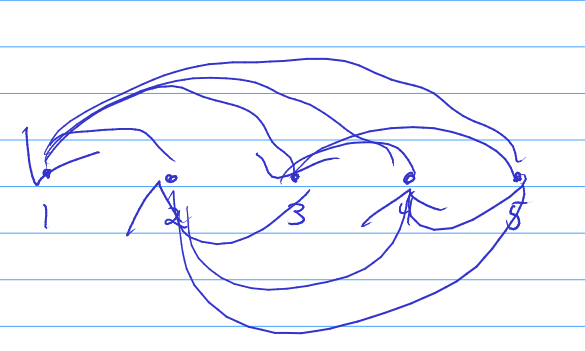
\includegraphics[width=0.7\textwidth]{images/11-01-01.png}
\end{figure}

\begin{prooflist}{2. Let $A=\{1,2,3,4,5,6\}$. Write out the relation $R$ that
		expresses $\mid$ (divides) on $A$. Then illustrate it with a diagram.}
	\item $R\subseteq A\times A = \set{(x, y): x\mid y}$.
\end{prooflist}
\begin{figure}
	\centering
	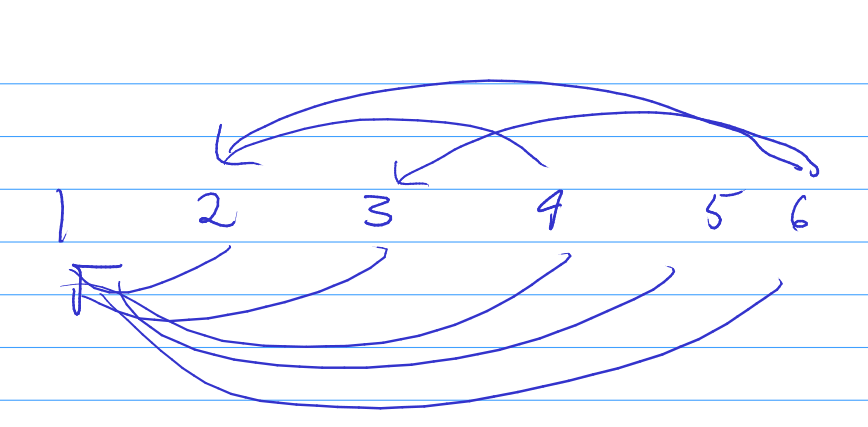
\includegraphics[width=0.7\textwidth]{images/11-01-02.png}
\end{figure}

\begin{prooflist}{3. Let $A=\set{0,1,2,3,4,5}$. Write out the relation $R$ that
		expresses $\geq$ on $A$. Then illustrate it with a diagram.}
	\item $R\subseteq A\times A = \set{(x, y): x-y \in \mathbb{N}}$.
	\item This relation defines a category. Take the diagram from the first
	problem and add identity arrows.
\end{prooflist}

\begin{prooflist}{4. Here is a diagram for a relation R on a set A. Write the sets A and R.}
	\item $A = \set{0, 1, 2, 3, 4, 5, 6}$
	\item $R\subseteq A\times A =$
	\item
	\begin{tabular}{l}
		(0, 0) \\
		(0, 4) \\
		(1, 1) \\
		(1, 3) \\
		(1, 5) \\
		(2, 2) \\
		(2, 4) \\
		(3, 1) \\
		(3, 3) \\
		(4, 0) \\
		(4, 2) \\
		(4, 4) \\
		(5, 1) \\
		(5, 5)
	\end{tabular}
\end{prooflist}
\begin{figure}
	\centering
	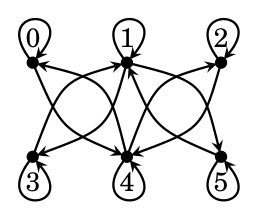
\includegraphics[width=0.4\textwidth]{images/11-01-04.png}
\end{figure}

\begin{prooflist}{5. Here is a diagram for a relation $R$ on a set $A$. Write the
		sets $A$ and $R$.}
	\item $A = \set{0, 1, 2, 3, 4, 5}$
	\item $R\subseteq A\times A =$
	\item
	\begin{tabular}{l}
		(1, 2) \\
		(2, 5) \\
		(3, 3) \\
		(4, 2) \\
		(4, 3) \\
		(5, 0)
	\end{tabular}
\end{prooflist}
\begin{figure}
	\centering
	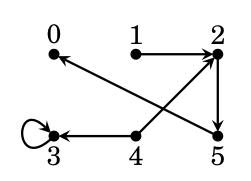
\includegraphics[width=0.4\textwidth]{images/11-01-05.png}
\end{figure}

\begin{prooflist}{6. Congruence modulo 5 is a relation on the set $A=\mathbb{Z}$. In this relation $x R y$ means $x \equiv y(\bmod 5)$. Write out the set $R$ in set-builder notation.}
	\item $R\subseteq A\times A = \set{(x, y) \in R: 5\mid x-y}$
\end{prooflist}

\begin{prooflist}{7. Write the relation $<$ on the set $A=\mathbb{Z}$ as a subset $R$ of $\mathbb{Z} \times \mathbb{Z}$. This is an infinite set, so you will have to use set-builder notation.}
	\item $R\subseteq A\times A = \set{(x, y) \in R: y-x \in \mathbb{N}_{>0}}$
\end{prooflist}

\begin{prooflist}{8. Let $A=\{1,2,3,4,5,6\}$. Observe that $\varnothing
			\subseteq A \times A$, so $R=\varnothing$ is a relation on $A$. Draw a
		diagram for this relation.}
	\item A diagram for a relation would have as points all elements of the set $R$.
	Because $R$ has no elements, the diagram is the empty diagram.
\end{prooflist}

\begin{prooflist}{9. Let $A = \set{1,2,3,4,5,6}$. How many different relations are there on the set A?}
	\item This can be solved with the multiplication principle. There are 6 choices
	for two spots, therefore there are $6^2$ different pairs $A\times A$.
	\item A relation is any powerset of $A\times A$, therefore the problem is the
	equivalent of determining the cardinality of the powerset of $A\times A$,
	which is $2^{36}$.
\end{prooflist}

\begin{prooflist}{10. Consider the subset $R=(\mathbb{R} \times \mathbb{R})-\{(x, x): x \in \mathbb{R}\} \subseteq \mathbb{R} \times \mathbb{R}$. What familiar relation on $\mathbb{R}$ is this? Explain.}
	\item This is the $\neq$ relation. We start with the full relation $\mathbb{R}
		\times \mathbb{R}$, and then substract all elements where the two elements
	are equal.  The universe minus the set where elements are equal leaves the
	unequal elements, therefore the $\neq$ relation.
\end{prooflist}

\begin{prooflist}{11. Given a finite set $A$, how many different relations are there on $A$ ?}
	\item Let us suppose we are only considering binary relations. Then the total
	number of relations is $2^{|A|^2}$.
\end{prooflist}

\begin{prooflist}{12-14. In the following exercises, subsets $R$ of $\mathbb{R}^2=\mathbb{R} \times \mathbb{R}$ or $\mathbb{Z}^2=\mathbb{Z} \times \mathbb{Z}$ are indicated by gray shading. In each case, $R$ is a familiar relation on $\mathbb{R}$ or $\mathbb{Z}$. State it.}
	\item 12. $R\subseteq \mathbb{R}\times\mathbb{R}\mid {x>y}$
	\item 13. $R\subseteq \mathbb{R}\times\mathbb{R}\mid {x\neq y}$
	\item 14. $R\subseteq \mathbb{R}\times\mathbb{R}\mid {x<y, x,y\in\mathbb{Z}}$
	\item 15. $R\subseteq \mathbb{R}\times\mathbb{R}\mid {x=y, x,y\in\mathbb{Z},
			x\mid 3}$
	\begin{figure}
		\centering
		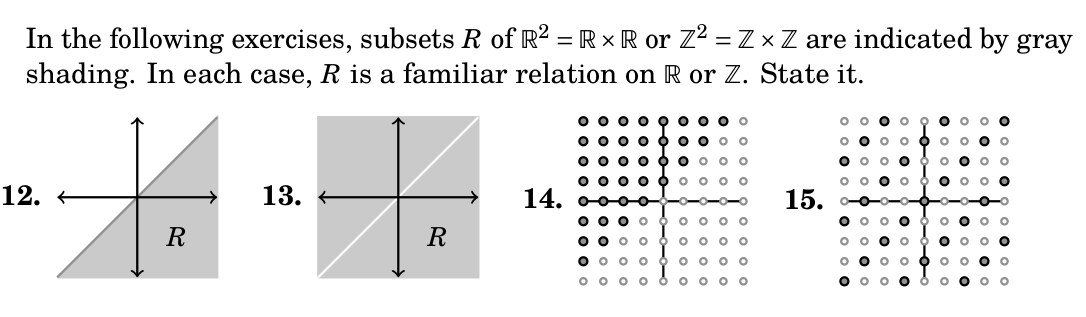
\includegraphics[width=0.9\textwidth]{images/11-01-12.png}
	\end{figure}
\end{prooflist}

\end{document}
